% -------------------------------------------------------------------------------------
\FloatBarrier
\section{Test su dati reali: la Crab osservata a Noto}
\label{sec:crabnoto}

Il test su B0329+54 (Sez.~\ref{sec:b0329}) riguarda un segnale lento e poco disperso, il caso sfavorevole per gli step 3 e
4. La pulsar della Crab (B0531+21, DM 56.7) è il caso opposto e il più vicino a un FRB: emette \emph{impulsi giganti}
singoli, stretti (decine di microsecondi) e fortemente dispersi. Il test usa anche un'antenna e un setup diversi da
quelli su cui la pipeline è stata sviluppata, quindi verifica pure che i valori di default non siano adattati a Medicina.

\subsection{Dati e pulizia}
Il file \file{n0325e_nt_no0005_IFall_vdif_pol2.fil} (Noto, 18 febbraio 2025) ha 1024 canali da \SI{0.25}{\mega\hertz}
(\SIrange{1350}{1606}{\mega\hertz}), campionamento di \SI{4}{\micro\second}, 8 bit e \SI{294}{\second} di durata
(\SI{75}{\giga\byte}). A DM 56.7 la dispersione attraversa la banda in circa \SI{38}{\milli\second}. La pipeline
(\file{tools/rfi_pipeline.py}, step 1--4, opzioni di default) ha impiegato \SI{4.7}{\hour}:
\begin{itemize}
  \item \textbf{step 1}: 100 canali mascherati, soprattutto il blocco \SIrange{1453}{1471}{\mega\hertz} (canali
    540--611, curtosi alta: RFI impulsivo), una ventina di canali a \SIrange{1521}{1563}{\mega\hertz} e alcuni a
    \SIrange{1364}{1382}{\mega\hertz}; 171 salti di guadagno; 0.03\% delle celle sostituite;
  \item \textbf{step 2}: una famiglia periodica a \SI{12.5}{\hertz} con 44 armoniche, sottratta;
  \item \textbf{step 3}: 9599 impulsi a DM 0, tutti rimossi, nessuno protetto; 1.7\% dei dati sostituiti;
  \item \textbf{step 4}: eccesso di rumore a DM 0 da 3.55 a 0.19 (a Medicina era 4.4--4.7), guadagno mediano 0.92.
    L'eccesso della differenza tra le due metà della banda resta 2.1: anche qui una parte della correlazione non è
    descritta da un solo modo comune.
\end{itemize}

\subsection{Impulsi giganti}
Il file originale e quello pulito sono stati cercati con \file{FRB_HF_Finder.py} (Heimdall + FETCH, DM 25--700,
soglia S/N 8, boxcar fino a 8192 campioni, modello \file{a}).

\paragraph{Identificazione dalla fase.} Per riconoscere gli impulsi giganti senza dipendere dalle soglie si usa la
periodicità della pulsar. I 30 candidati del file pulito con DM $56.72\pm0.2$ e FETCH\,$\geq$\,0.5 sono stati ripiegati
in tempo su una griglia di periodi (\SIrange{33.80}{33.88}{\milli\second}), massimizzando la statistica $Z^2_5$. Il
periodo topocentrico che li mette in fase è $P=\SI{33.84143}{\milli\second}$ ($Z^2_5=257$, contro 13 in mediana sulla
griglia): con questo periodo 28 impulsi cadono entro $\pm0.015$ in fase (impulso principale) e 2 a $+0.40$
(interimpulso), come atteso per la Crab (Fig.~\ref{fig:crabnoto}, a sinistra). Il periodo baricentrico corrispondente,
circa \SI{33.838}{\milli\second}, è coerente con la rotazione della Crab estrapolata a febbraio 2025.
\ipotesi{Il confronto con l'effemeride usa valori di frequenza e derivata citati a memoria; va verificato con
l'effemeride mensile di Jodrell Bank.} Si conta come impulso gigante ogni candidato con DM entro 1 da 56.72 e fase
entro 0.03 dall'impulso principale o dall'interimpulso: a quella DM, fuori fase, c'è un solo candidato per file.

\begin{table}[ht]
\centering
\caption{Ricerca con \file{FRB_HF_Finder.py} sul file originale e su quello pulito (step 1--4).}
\label{tab:crabnoto}
\small
\begin{tabular}{lcc}
\toprule
 & originale & pulito \\
\midrule
candidati Heimdall (DM 25--700) & 575 & 338 \\
impulsi giganti (in fase, DM $56.72\pm1$) & 28 & \textbf{43} \\
\quad di cui con FETCH\,$\geq$\,0.5 & 13 & \textbf{30} \\
candidati che non sono la Crab & 547 & 295 \\
\quad a DM 25--50 & 124 & 55 \\
\quad con boxcar $\geq2^{12}$ campioni & 157 & 263 \\
\quad con FETCH\,$\geq$\,0.5 & 0 & 0 \\
\midrule
impulsi giganti in comune & \multicolumn{2}{c}{26} \\
S/N pulito / originale (mediana; intervallo) & \multicolumn{2}{c}{1.17;\; 0.91--2.06} \\
\bottomrule
\end{tabular}
\end{table}

\paragraph{Risultati} (Tab.~\ref{tab:crabnoto}, Fig.~\ref{fig:crabnoto}).
\begin{itemize}
  \item \textbf{Più impulsi rivelati.} Gli impulsi giganti passano da 28 a 43, quelli accettati da FETCH da 13 a 30.
    Dei 28 dell'originale, 26 sono trovati anche nel file pulito; i 2 persi sono vicini alla soglia (S/N 8.3--8.4) e
    FETCH li scartava già. Dopo la pulizia compaiono 17 impulsi nuovi.
  \item \textbf{Nessuna perdita di segnale.} Per i 26 impulsi in comune l'S/N migliora in mediana del 17\%, senza casi
    di perdita significativa (minimo 0.91). Lo step 3 non ha protetto nessun evento e non ha comunque toccato gli
    impulsi: lo sweep di \SI{38}{\milli\second} li distingue nettamente dall'RFI a DM 0. Anche lo step 4, che perde
    circa larghezza/sweep del segnale (Sez.~\ref{sec:step4}), qui perde meno dell'1\%. È la verifica complementare a
    B0329+54: su segnali stretti e dispersi, cioè su FRB tipici, la pipeline conserva il segnale e riduce il rumore.
  \item \textbf{FETCH.} Nell'originale FETCH scartava anche impulsi forti (S/N 12.1 a \SI{67.4}{\second}, 18.3 a
    \SI{204.2}{\second} con probabilità 0.44), probabilmente perché l'RFI nelle immagini lo confondeva; nel file pulito
    li accetta. Restano scartati 13 impulsi veri, tutti con S/N fra 8.1 e 11.6 e quasi sempre con probabilità sotto
    0.05: vicino alla soglia FETCH non riconosce il segnale. Con FETCH a 0.7 la ricerca è quindi di fatto completa solo
    sopra S/N circa 11--12, non dalla soglia di Heimdall.
  \item \textbf{Falsi candidati.} I candidati che non sono la Crab si dimezzano (da 547 a 295); a DM 25--50 calano da
    124 a 55. Nel file pulito sono quasi tutti (263) con boxcar di $2^{12}$--$2^{13}$ campioni, al limite di Heimdall:
    la stessa popolazione vista a Medicina anche nel file di solo rumore (Sez.~\ref{sec:completeness}). Nell'originale
    c'erano molti più candidati con larghezze intermedie, dovuti all'RFI. Nessun falso positivo FETCH in entrambi i casi.
\end{itemize}

\begin{figure}[ht]
\centering
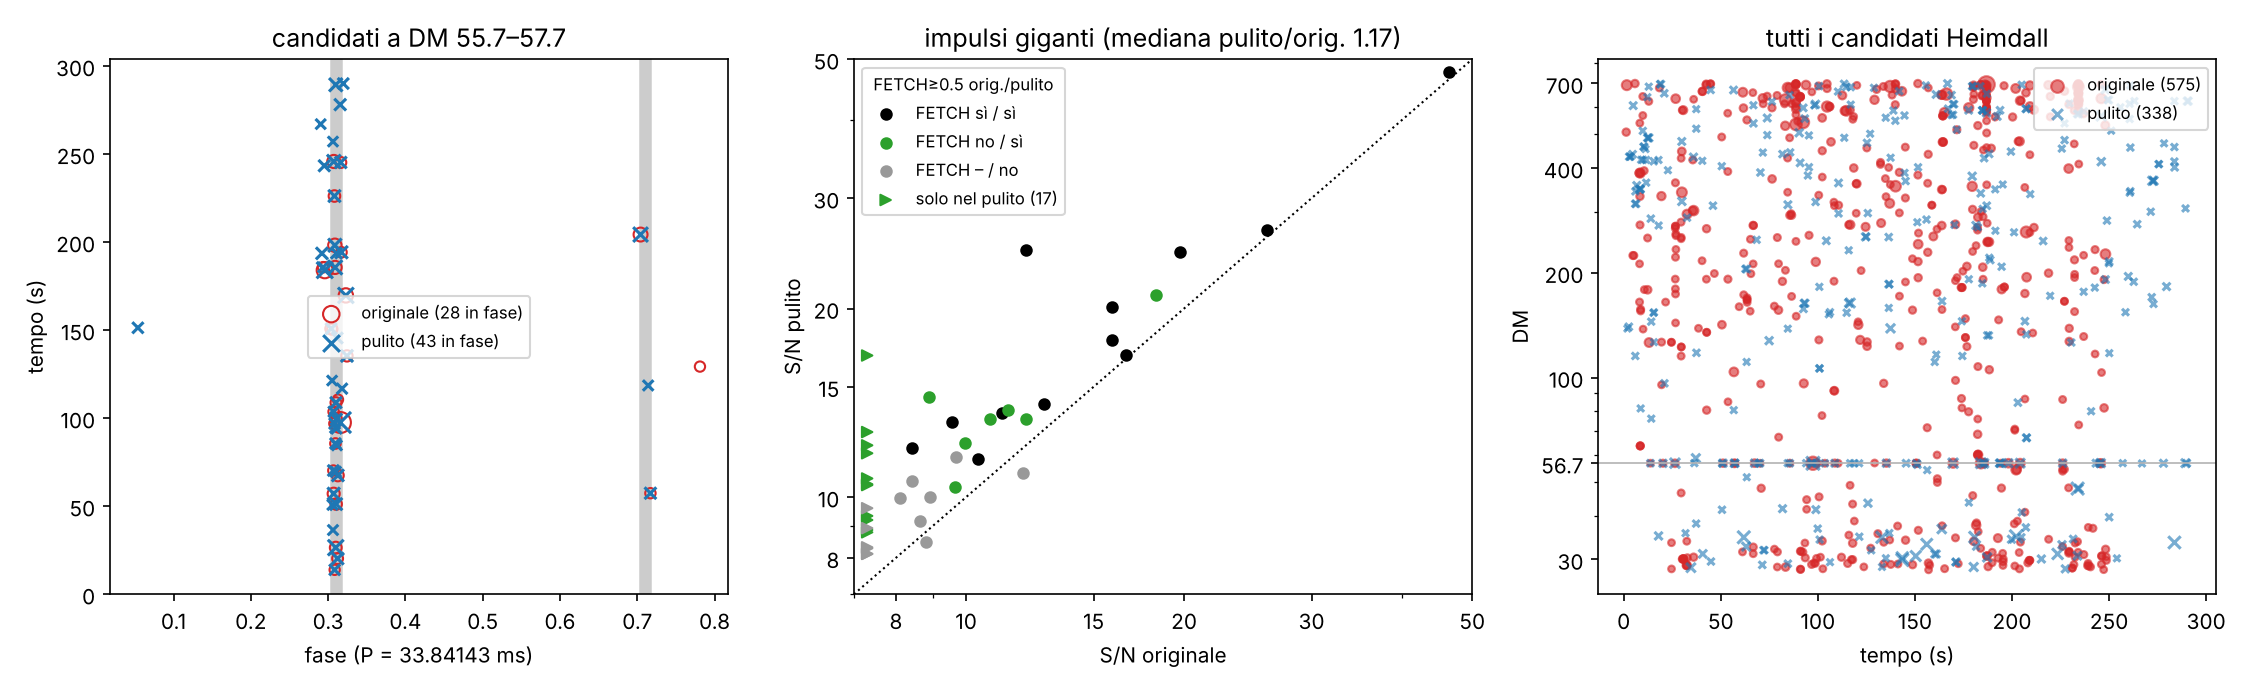
\includegraphics[width=\textwidth]{fig/pipeline/crab_noto_gp.png}
\caption{Crab a Noto, ricerca con \file{FRB_HF_Finder.py} sul file originale (rosso) e pulito (blu). Sinistra: fase
dei candidati a DM 55.7--57.7 per $P=\SI{33.84143}{\milli\second}$ (in grigio le finestre dell'impulso principale e
dell'interimpulso); la dimensione è proporzionale all'S/N. Centro: S/N degli impulsi giganti nel file pulito rispetto
all'originale, con la classificazione FETCH ($\geq0.5$) nei due file; i triangoli a sinistra sono gli impulsi trovati
solo nel file pulito. Destra: tutti i candidati Heimdall nel piano tempo--DM.}
\label{fig:crabnoto}
\end{figure}

\subsection{Un impulso gigante prima e dopo la pulizia}
La Fig.~\ref{fig:crabgp} mostra, con \file{tools/plot_dynspec.py}, \SI{120}{\milli\second} attorno all'impulso gigante
più forte (\SI{97.474}{\second}, S/N 47.6), a DM 0, nel file originale e dopo lo step 4, con la stessa scala di colori.
\begin{itemize}
  \item \textbf{Originale.} La serie a DM 0 è dominata dai lampi della banda \SIrange{1445}{1480}{\mega\hertz} (a circa
    20, 30, 40 e \SI{100}{\milli\second}, alti 2--3 conteggi), che nello spettro dinamico sono blocchi chiari; nella
    stessa banda strisce verticali fitte alternano livelli alti e bassi. Lo spettro medio mostra le portanti a
    \SIrange{1525}{1555}{\mega\hertz} e la depressione del bandpass a \SIrange{1453}{1471}{\mega\hertz}. L'impulso
    gigante è la traccia diagonale debole da circa \SI{55}{\milli\second} (\SI{1606}{\mega\hertz}) a circa
    \SI{92}{\milli\second} (\SI{1350}{\mega\hertz}); nella serie a DM 0 non si vede.
  \item \textbf{Dopo lo step 4.} La serie a DM 0 è piatta, lo spettro medio è piatto, i lampi e le portanti sono
    spariti, il blocco \SIrange{1453}{1471}{\mega\hertz} e i canali a \SI{1381}{\mega\hertz} sono mascherati (rosa).
    La traccia dell'impulso gigante resta intatta ed è ora la struttura più evidente del pannello.
\end{itemize}
È l'illustrazione diretta di quanto misurato con la ricerca: la pulizia rimuove l'RFI a DM 0 e il rumore comune senza
toccare un segnale stretto e disperso.

\begin{figure}[ht]
\centering
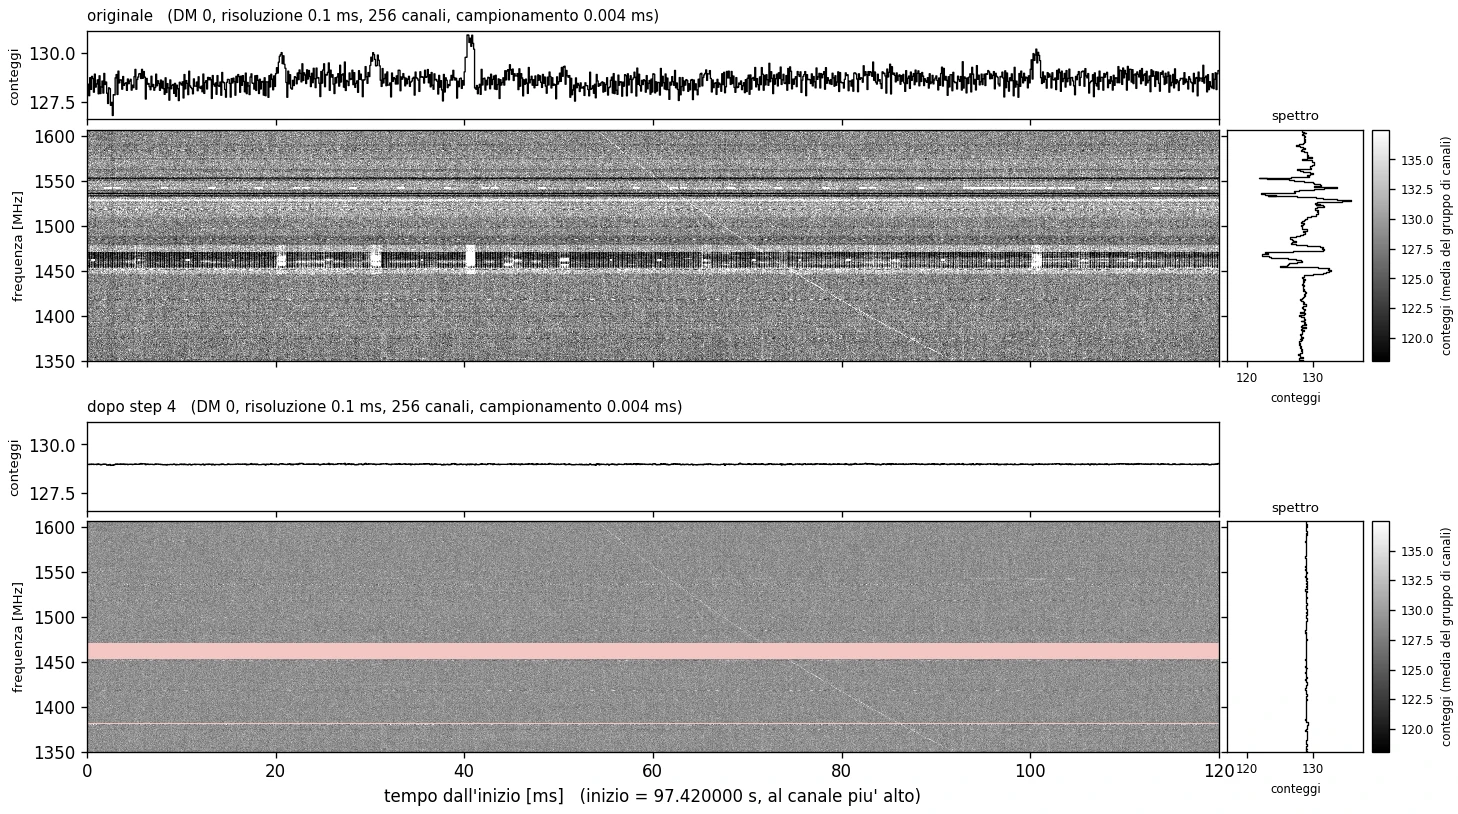
\includegraphics[width=\textwidth]{fig/noto/crab_gp97_dm0.png}
\caption{L'impulso gigante più forte della Crab a Noto (\SI{97.474}{\second}, DM 56.7, S/N 47.6), a DM 0, nel file
originale (sopra) e dopo lo step 4 (sotto): \SI{120}{\milli\second} da \SI{97.42}{\second}, risoluzione
\SI{0.1}{\milli\second}, 256 canali, stessa scala di colori in conteggi. Per ciascun file: serie temporale, spettro
dinamico e spettro medio sulla finestra. Rosa: canali mascherati.}
\label{fig:crabgp}
\end{figure}

\subsection{Ripiegamento e ricerca a singolo impulso con PRESTO}
\sloppy
\begin{itemize}
  \item \textbf{Ripiegamento.} I ripiegamenti con \file{prepfold -psr B0531+21} non mostrano la pulsar in nessuno step.
    Il periodo dato dall'effemeride di TEMPO, \SI{33.84828}{\milli\second}, differisce da quello misurato dagli impulsi
    giganti di \SI{0.0069}{\milli\second} ($2\times10^{-4}$): in \SI{294}{\second} la fase scivola di circa 1.8 giri e
    il profilo si appiattisce. Il parfile usato non è aggiornato: per la Crab, con forte rumore di timing e glitch,
    serve l'effemeride mensile. Il ripiegamento con ricerca in periodo sull'originale ($\chi^2_{\rm red}=47$) e quello a
    parametri fissi ($\chi^2_{\rm red}=15.8$) sono dominati dall'RFI: il primo converge a
    $\dot P=\num{-1.3e-7}$, non fisico, e il secondo scende a $\chi^2_{\rm red}\simeq1.5$ sia con la maschera di
    \file{rfifind} sia dopo lo step 1.
  \item \textbf{Ripiegamento al periodo degli impulsi giganti.} Il periodo ricavato dagli impulsi giganti è
    topocentrico, mentre \file{prepfold -p} lo interpreta come baricentrico se l'header contiene le coordinate: serve
    l'opzione \file{-topo}. Con \file{-topo -nosearch}, $P=\SI{33.841426}{\milli\second}$, DM 56.72 e 128 intervalli,
    la Crab compare negli step 1, 2 e 3: un impulso stretto (un intervallo, \SI{0.26}{\milli\second}) alla stessa fase
    degli impulsi giganti, con un rilievo a DM\,$\simeq$\,56.7 nella curva DM. L'impulso in un solo intervallo
    conferma il periodo entro circa \SI{3e-5}{\milli\second}. La misura dell'S/N del profilo per ogni step è nella
    Tab.~\ref{tab:crabprof} e nella Fig.~\ref{fig:crabprof}.
  \item \textbf{Un picco spurio vicino al periodo della Crab.} Dopo lo step 1 la curva $\chi^2$--periodo di
    \file{prepfold} ha un picco a $P\simeq\SI{33.8459}{\milli\second}$, più alto di quello della pulsar; dopo lo step 2
    scompare e resta solo il picco della Crab. È la famiglia periodica a \SI{12.5}{\hertz} sottratta dallo step 2: la
    sua 26ª armonica (\SI{325}{\hertz}, presente fra le righe trovate) coincide con l'11ª armonica della frequenza di
    ripiegamento, $12.5\times26/11=\SI{29.5454}{\hertz}$, cioè $P=\SI{33.8462}{\milli\second}$. Non è una coincidenza
    fisica: in una finestra di ricerca stretta, attorno a qualunque periodo, qualche armonica di un treno ricco di
    armoniche trova un'armonica del ripiegamento. Senza lo step 2 una ricerca in periodo si sarebbe agganciata all'RFI.
  \item \textbf{S/N del profilo per ogni step} (Tab.~\ref{tab:crabprof}, Fig.~\ref{fig:crabprof}). Stesso metodo di
    B0329+54: segnale integrato sui 3 intervalli dell'impulso principale diviso il rumore robusto fuori impulso. Il
    rumore è confrontato con quello bianco atteso da \file{prepfold} (\emph{Profile StdDev}, dalla deviazione standard
    dei dati) e, per gli step 1--4, con quello radiometrico ($8\sqrt{924}\sqrt{N_{\rm campioni/bin}}$ conteggi).
    \begin{itemize}
      \item Nell'originale il profilo è dominato da variazioni lente dovute all'RFI (rumore 2.3 volte quello bianco):
        S/N 4.4. La maschera di \file{rfifind} e lo step 1 lo portano a 9--10, con rumore vicino a quello bianco.
      \item Gli step 1--3 conservano tutto il segnale (rapporto con lo step 2: 1.01, 1.00, 1.00), e lo step 4 anche
        (0.996), come previsto per un impulso stretto (Sez.~\ref{sec:step4}); è l'opposto di B0329+54 (0.07).
      \item Lo step 4 aumenta però leggermente il rumore del profilo (da 1.29 a 1.45 volte il radiometrico), e l'S/N
        scende da 9.5 a 8.4. La differenza è al limite dell'incertezza della stima del rumore (circa 7\% con circa
        110 intervalli fuori impulso). Qui il rumore del profilo è già vicino al radiometrico dopo lo step 1, quindi lo
        step 4 non ha nulla da guadagnare sul ripiegamento; il suo guadagno è sulla ricerca a singolo impulso.
      \item La maschera di \file{rfifind} dà sul ripiegamento lo stesso risultato della pipeline (9.7 contro 9.5--9.8):
        per il segnale medio di una pulsar la differenza fra i due metodi è trascurabile. La differenza è negli impulsi
        singoli (Tab.~\ref{tab:crabnoto}).
      \item L'interimpulso non è rivelato (meno di 2$\sigma$ in tutti i file).
    \end{itemize}
  \item \textbf{Ricerca a singolo impulso.} Con \file{prepsubband} (DM 30--85, passo 1) e \file{single_pulse_search.py}
    gli eventi passano da 6227 (5260 a DM\,$<$\,50) nell'originale a 111 (27 a DM\,$<$\,50) nel file pulito. Gli
    impulsi giganti sono trovati però con S/N basso (massimo 9.4): con \SI{256}{\mega\hertz} di banda un errore di 0.5
    in DM sbava l'impulso di circa \SI{0.3}{\milli\second}, contro una durata di circa \SI{0.05}{\milli\second}. Per un
    confronto equo serve un passo di circa 0.05 attorno a DM 56.7.
\end{itemize}
\fussy


\begin{table}[ht]
\centering
\caption{Crab a Noto, ripiegamento a $P=\SI{33.841426}{\milli\second}$ (topocentrico), DM 56.72, 128 intervalli: S/N
del profilo (impulso principale, 3 intervalli), rumore fuori impulso rispetto al bianco atteso da \file{prepfold} e al
radiometrico, segnale integrato rispetto allo step 2.}
\label{tab:crabprof}
\small
\begin{tabular}{lccccc}
\toprule
 & S/N del picco & S/N integrato & rumore / bianco & rumore / radiometrico & segnale / step 2 \\
\midrule
originale & 3.7 & 4.4 & 2.26 & -- & -- \\
originale + \file{rfifind} & 8.7 & 9.7 & 1.02 & -- & -- \\
step 1 & 7.8 & 9.1 & 1.14 & 1.37 & 1.01 \\
step 2 & 8.6 & 9.8 & 1.04 & 1.25 & 1.00 \\
step 3 & 8.3 & 9.5 & 1.08 & 1.29 & 1.00 \\
step 4 & 7.4 & 8.4 & 1.21 & 1.45 & 1.00 \\
\bottomrule
\end{tabular}
\end{table}

\begin{figure}[ht]
\centering
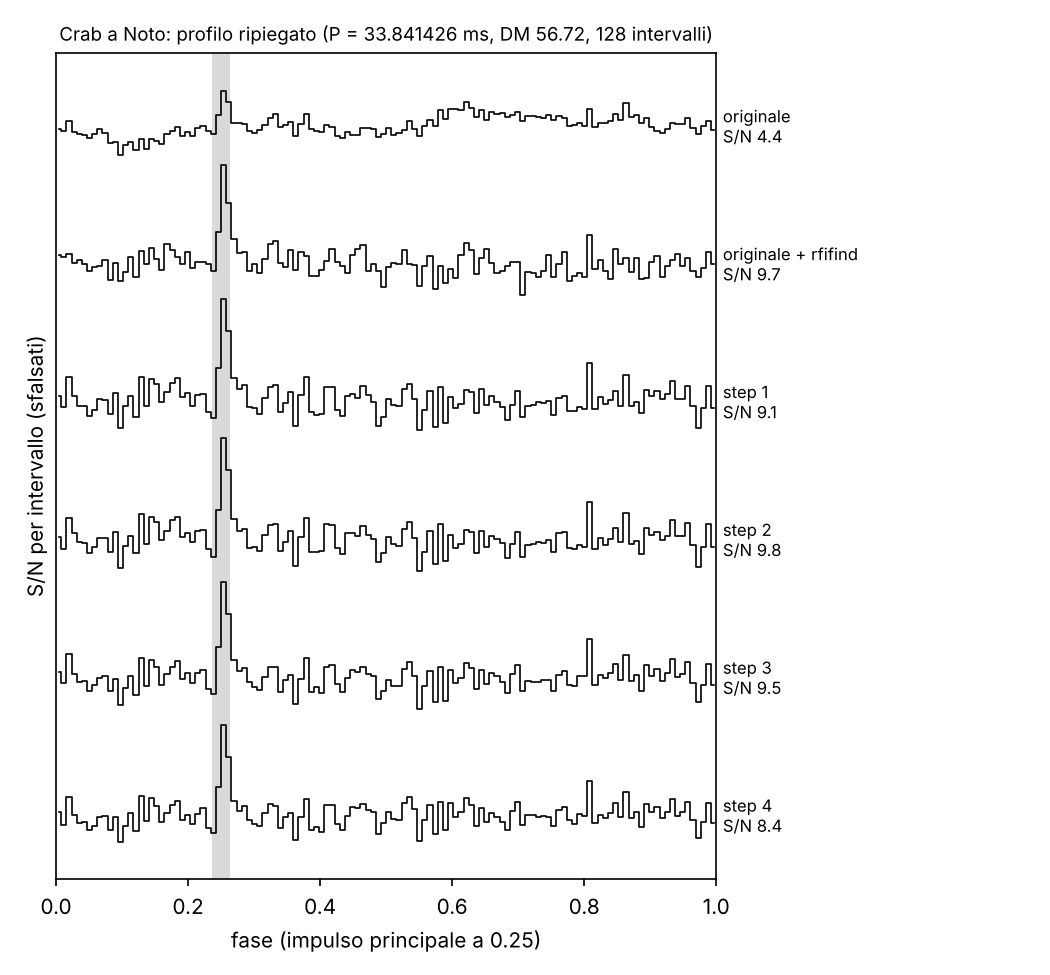
\includegraphics[width=0.75\textwidth]{fig/noto/crab_profiles.png}
\caption{Profili della Crab a Noto (\SI{294}{\second}, 128 intervalli) nel file originale, con la maschera di
\file{rfifind} e dopo ogni step, ciascuno in unità del proprio rumore fuori impulso e sfalsati in verticale. In grigio la
finestra dell'impulso principale usata per l'S/N.}
\label{fig:crabprof}
\end{figure}

% -------------------------------------------------------------------------------------
\subsection{L'ambiente RFI di Noto in banda L}
\label{sec:notoenv}
Il file originale e quello pulito sono stati analizzati con \file{tools/rfi_survey.py} (opzioni di default, con lo
spettro di potenza della serie a DM 0 alla risoluzione nativa, fino a \SI{125}{\kilo\hertz}). È una sola osservazione di
\SI{294}{\second}: il quadro è indicativo, e le identificazioni delle sorgenti sono ipotesi.

\paragraph{Cosa contiene il file originale} (Figg.~\ref{fig:notodyn} e \ref{fig:notospec}).
\begin{itemize}
  \item \textbf{Banda \SIrange{1445}{1495}{\mega\hertz}: la sorgente dominante.} Lampi di qualche secondo, a gruppi,
    per tutta l'osservazione, alternati a fasi in cui il livello scende sotto la mediana. Le stesse fasi producono le
    cadute verso il basso della serie a DM 0 (fino a circa $-8\%$ della potenza totale, a
    \SIrange{130}{160}{\second} e \SIrange{205}{265}{\second}). Nella stessa banda, a \SIrange{1478}{1494}{\mega\hertz},
    c'è un treno di impulsi larghi \SI{0.5}{\milli\second} a \SI{12.5}{\hertz} (4435 eventi, statistica di Rayleigh
    $Z=2408$), la famiglia sottratta dallo step 2. \ipotesi{\SIrange{1452}{1492}{\mega\hertz} è la banda europea della
    telefonia mobile in sola discesa (SDL): un segnale digitale a trame regolari è compatibile. La discesa del livello
    all'arrivo di un segnale forte fa pensare a un controllo automatico del guadagno nel ricevitore o nel backend.}
  \item \textbf{Banda \SIrange{1505}{1575}{\mega\hertz}.} Portanti strette persistenti a \SIrange{1525}{1555}{\mega\hertz},
    con molti valori estremi e livello molto variabile, e una struttura lenta e larga: fra circa 150 e
    \SI{230}{\second} il livello di tutta la banda scende per circa \SI{80}{\second}. \ipotesi{\SIrange{1525}{1559}{\mega\hertz}
    è la banda di discesa dei satelliti per comunicazioni mobili (per esempio Inmarsat).}
  \item \textbf{Portante a \SI{1437}{\mega\hertz}}, stretta e intermittente (\SIrange{8}{70}{\second} e
    \SIrange{190}{250}{\second}).
  \item \textbf{Righe periodiche.} Oltre a \SI{12.5}{\hertz}, righe a 2, 9.5 e \SI{33.3}{\hertz}; nel kHz una famiglia
    a multipli di \SI{2}{\kilo\hertz} (armoniche di \SI{200}{\hertz} fino a \SI{12}{\kilo\hertz}) e righe isolate a 22,
    42, 46, 50, \SI{52}{\kilo\hertz} e oltre, 60 in tutto. \ipotesi{Righe di questo tipo sono tipiche di elettronica
    locale (alimentatori, clock digitali).}
  \item \textbf{Eventi impulsivi a DM 0.} 7623, quasi tutti in una sola sottobanda: 7620 colpiscono al più il 25\% della
    banda, nessuno più del 75\%. S/N massimo 35; 106 eventi con S/N\,$\geq$\,20.
  \item \textbf{Bandpass e guadagno.} Il bandpass è già piatto in ingresso (circa 123 conteggi): il backend equalizza
    la banda, e la sua forma reale non è ricostruibile. 171 salti di guadagno, a intervalli irregolari.
\end{itemize}

\begin{table}[ht]
\centering
\caption{Ambiente RFI in banda L: Medicina (Sez.~\ref{sec:rfienv}) e Noto (questa sezione).}
\label{tab:notoenv}
\small
\begin{tabular}{p{4.2cm}p{4.6cm}p{5.4cm}}
\toprule
 & Medicina & Noto \\
\midrule
radar a banda larga & due, periodo \SI{10}{\second}, dominanti & nessun evento a banda larga \\
rete elettrica & famiglia a \SI{50}{\hertz} & non evidente \\
treni periodici & \SI{1.987}{\hertz} & \SI{12.5}{\hertz}, impulsi da \SI{0.5}{\milli\second} a \SIrange{1478}{1494}{\mega\hertz} \\
righe nel kHz & -- & famiglia a \SI{2}{\kilo\hertz}, righe a \SIrange{22}{52}{\kilo\hertz} \\
RFI in banda & \SIrange{1438}{1440}{\mega\hertz}, \SI{1421}{\mega\hertz} & \SIrange{1445}{1495}{\mega\hertz} (forte),
  \SIrange{1525}{1555}{\mega\hertz}, \SI{1437}{\mega\hertz} \\
eccesso di rumore a DM 0 & 4.4--4.7 & 3.5 (2.5--5.0 fra i blocchi) \\
salti di guadagno & circa ogni \SI{1}{\second} & 171 in \SI{294}{\second}, irregolari \\
\bottomrule
\end{tabular}
\end{table}

\paragraph{Confronto con Medicina} (Tab.~\ref{tab:notoenv}). L'RFI di Noto è soprattutto a banda stretta e
compatibile con servizi di telecomunicazione; a Medicina dominano radar e disturbi locali a banda larga. Il rumore
correlato fra i canali c'è in entrambi i siti, a Noto un po' minore, e anche qui la differenza fra le due metà della
banda (eccesso 2.1) non è descritta da un solo modo comune.

\paragraph{Dopo la pipeline} (Fig.~\ref{fig:notodyn}, sotto). Spariscono il treno a \SI{12.5}{\hertz} (Rayleigh da
1619 a 2.6 su tutti gli eventi), quasi tutte le righe dello spettro (da 60 a 2, al limite della soglia: \SI{2125.85}{\hertz}
e \SI{91.56}{\kilo\hertz}, quest'ultima con periodo di 2.7 campioni, sotto il minimo dello step 2) e gli eventi forti
(S/N\,$\geq$\,20 da 106 a 0, S/N\,$\geq$\,10 da 2000 a 149). Restano:
\begin{itemize}
  \item i \textbf{bordi del blocco mascherato}, \SIrange{1446}{1452}{\mega\hertz} e \SIrange{1472}{1480}{\mega\hertz}: i
    lampi vi sono ancora visibili nel pannello del massimo, e lo step 4 vi trova i guadagni più alti (1.6--1.9 contro
    0.92 in mediana);
  \item impulsi deboli non periodici a \SIrange{1414}{1430}{\mega\hertz} (863 eventi);
  \item le portanti a \SIrange{1525}{1555}{\mega\hertz} e la struttura lenta a \SIrange{1505}{1575}{\mega\hertz}.
\end{itemize}
Sono due limiti dello step 1. (1) Il rumore di ogni canale è confrontato con la mediana dei circa 32 canali vicini: se
un blocco di RFI è largo quanto metà di questa finestra, il riferimento è contaminato e i canali ai bordi sembrano
normali. (2) Ogni canale è riassunto dalla \emph{mediana nel tempo} delle sue statistiche: un RFI presente in meno di
metà dei blocchi non la sposta, per quanto sia forte. I rimedi, che usano statistiche già calcolate, sono un secondo
passaggio della maschera con i riferimenti ricalcolati senza i canali già mascherati e un criterio per l'RFI
intermittente (un percentile alto nel tempo invece della mediana, o la variabilità del livello fra i blocchi). Va
evitato di mascherare la riga dell'idrogeno a \SI{1420.4}{\mega\hertz}, forte in direzione della Crab, che non è RFI.

\begin{figure}[p]
\centering
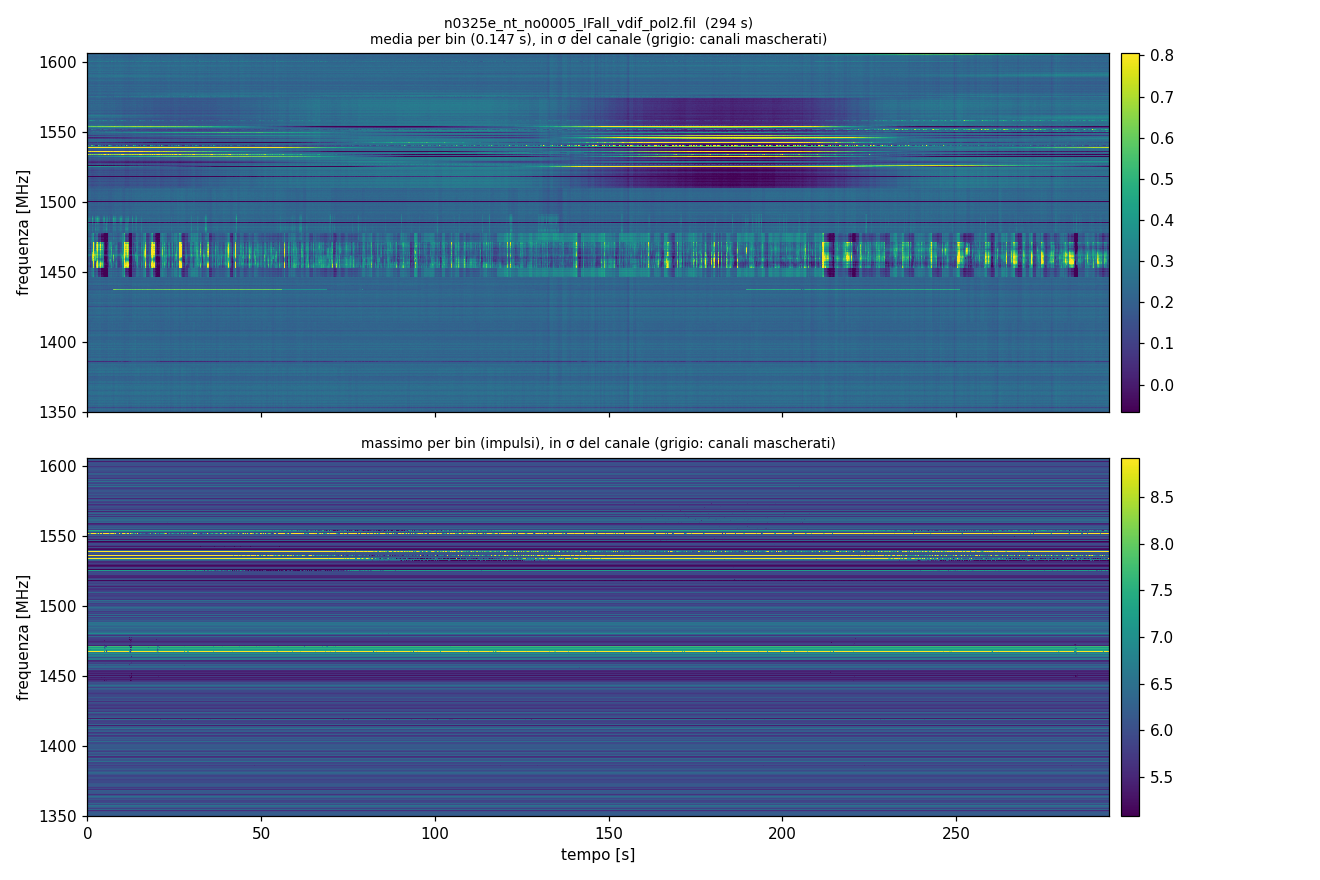
\includegraphics[width=\textwidth]{fig/noto/survey_orig_dynspec.png}\\[2mm]
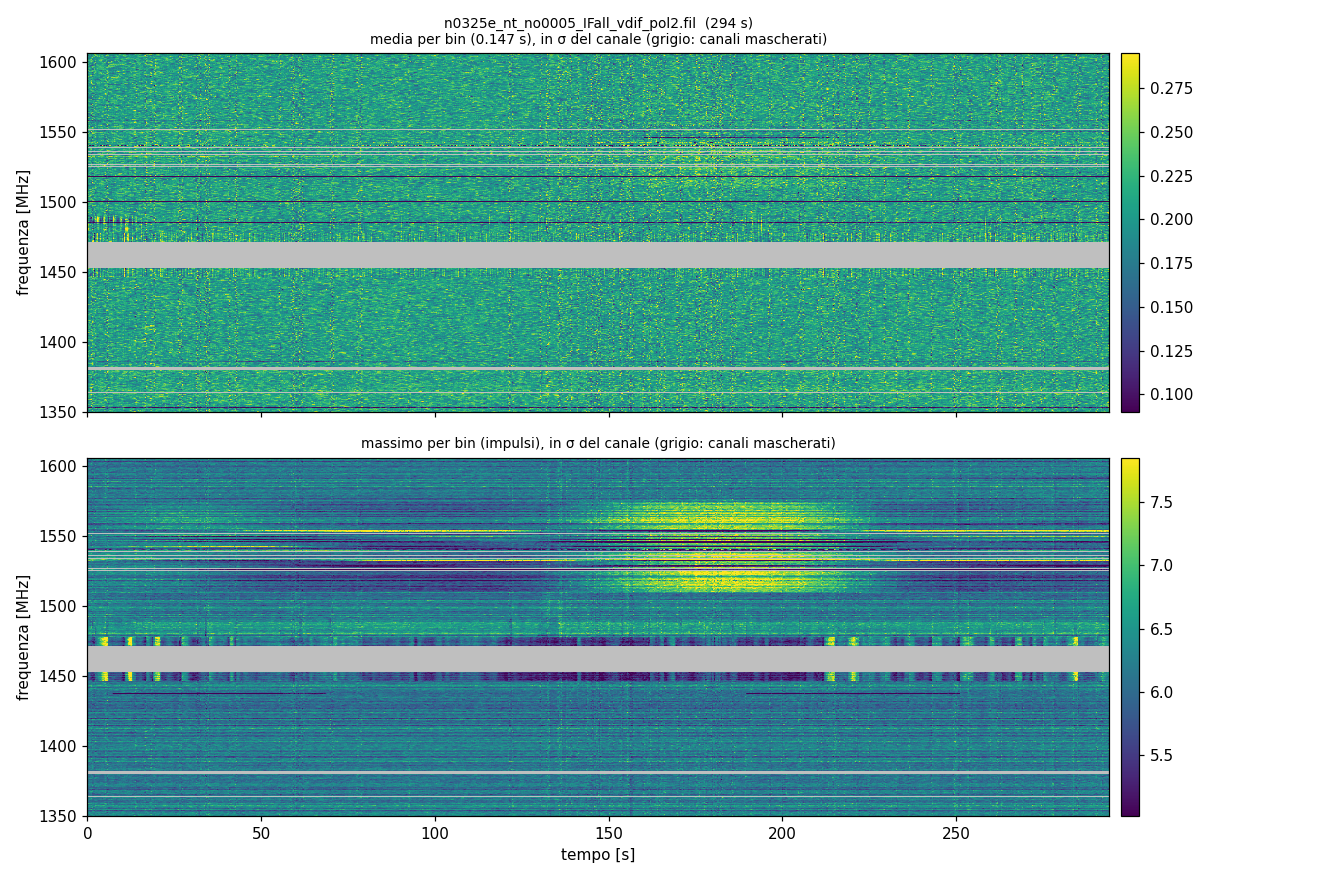
\includegraphics[width=\textwidth]{fig/noto/survey_clean_dynspec.png}
\caption{Censimento di Noto (\file{rfi_survey.py}): spettri dinamici di tutta l'osservazione (\SI{294}{\second},
intervalli di \SI{0.147}{\second}), in unità della $\sigma$ di ciascun canale, nel file originale (sopra) e dopo gli
step 1--4 (sotto). Per ciascuno: media per intervallo (variazioni di livello) e massimo per intervallo (impulsi).
Grigio: canali mascherati.}
\label{fig:notodyn}
\end{figure}

\begin{figure}[ht]
\centering
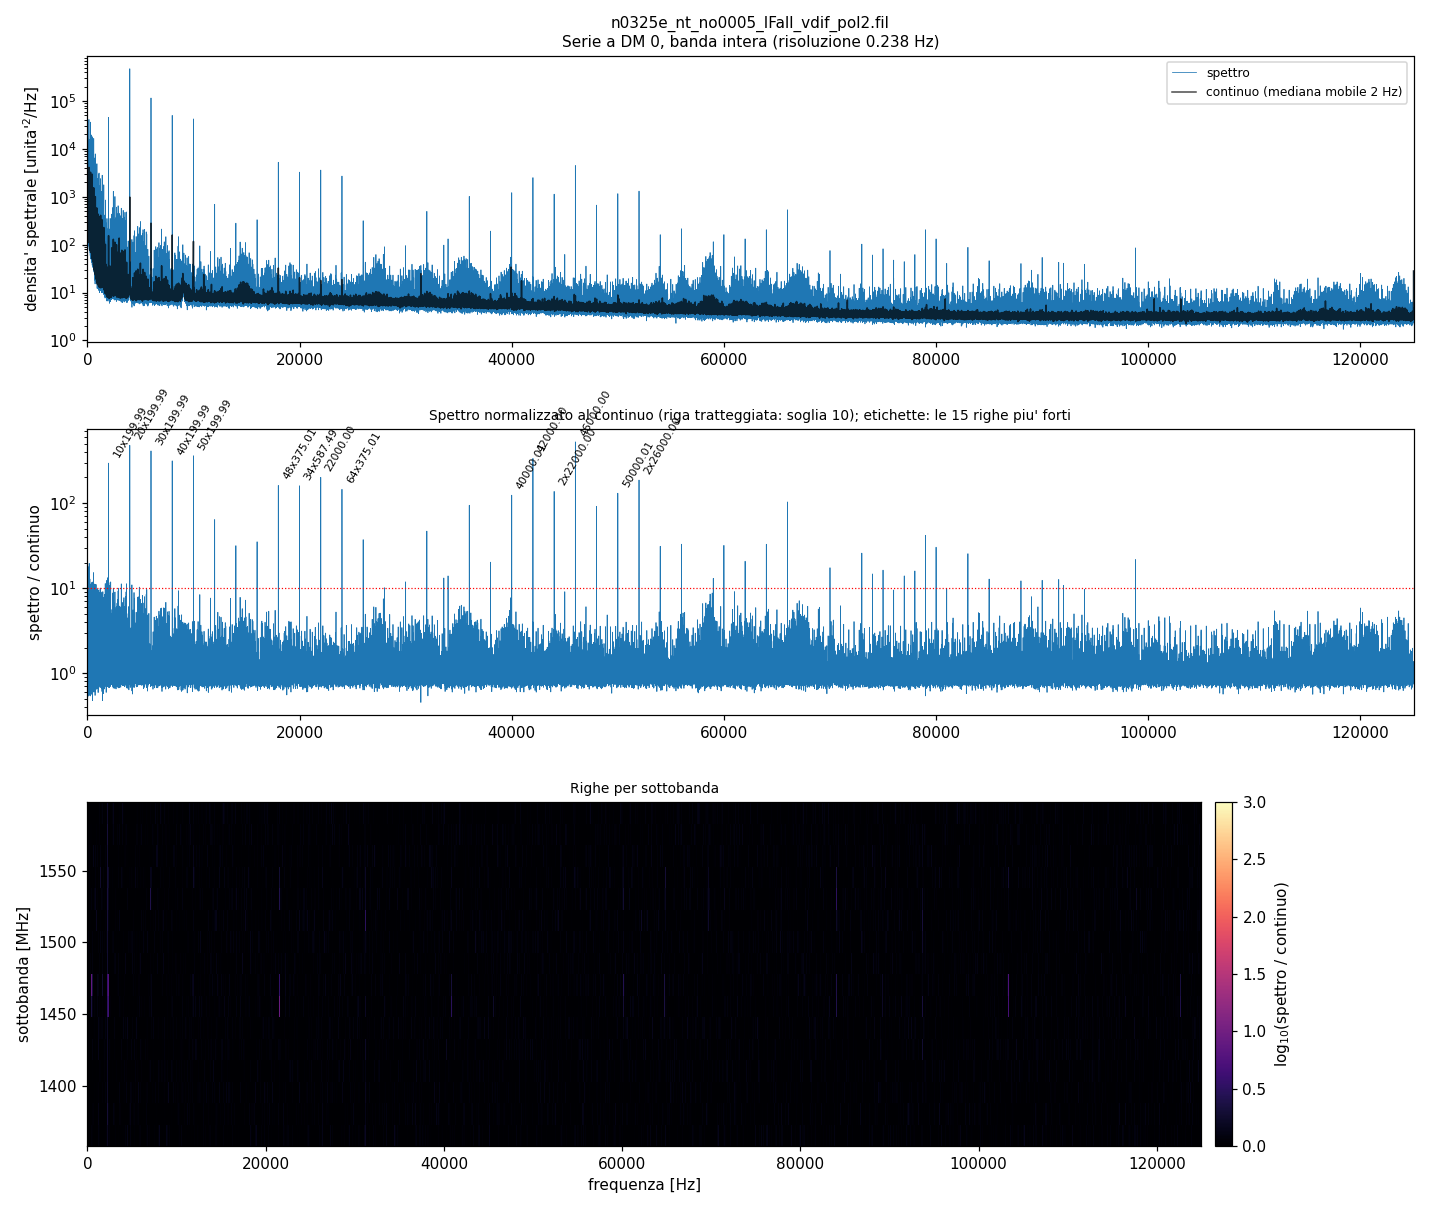
\includegraphics[width=\textwidth]{fig/noto/survey_orig_spectrum.png}
\caption{Spettro di potenza della serie a DM 0 del file originale di Noto (risoluzione \SI{0.24}{\hertz}, fino a
\SI{125}{\kilo\hertz}): spettro e continuo, spettro normalizzato al continuo con le righe più forti, righe per
sottobanda. Dopo la pipeline restano 2 righe al limite della soglia.}
\label{fig:notospec}
\end{figure}
